\RequirePackage[l2tabu, orthodox]{nag}
\documentclass[12pt]{article}
\usepackage[T1]{fontenc}
\usepackage{fontspec}
% \setmainfont{Latin Modern Roman}
\usepackage[utf8]{inputenc}
\usepackage[french]{babel}
\usepackage{amsthm,amssymb,amsmath,xcolor}
\usepackage{setspace}
% \doublespacing
\usepackage{geometry}
\geometry{
    a4paper,
    total={170mm,257mm},
}
\usepackage{graphicx}
\graphicspath{ {./} }
\usepackage{microtype}
\usepackage{todonotes}
\usepackage{hyperref}
\hypersetup{
    colorlinks=true,
    linkcolor=blue,
    filecolor=magenta,
    urlcolor=cyan,
    breaklinks=true,
    pdftitle={Rapport PSAR Orchestration de micro-vm via un resolver DNS},
    pdfauthor={Efe ERKEN},
    pdfencoding=auto, % Helps with unicode in bookmarks/metadata
    unicode=true % Enable unicode support
}
\usepackage[indent]{parskip}
\usepackage{float}
\usepackage{wrapfig}
\usepackage{listings} % Ajout pour les blocs de code
% Fix quotes: Use csquotes package
\usepackage[autostyle=true, style=french]{csquotes} % Recommended for quotes in french
\MakeOuterQuote{"}

\lstset{ % Configuration globale pour listings
    basicstyle=\footnotesize\ttfamily,
    breaklines=true,
    postbreak=\mbox{\textcolor{red}{$\hookrightarrow$}\space},
}

\author{Efe ERKEN}
\date{\today}
\title{Rapport PSAR  \\ ``Orchestration de micro-vm via un resolver DNS''}

\begin{document}
\maketitle

\begin{abstract}
	Dans le cadre de l'UE "Projet Systèmes et Applications Répartie" (PSAR) du master informatique parcours SAR du même nom à la Sorbonne Université, nous devions choisir un sujet de projet programmation parmi une dizaine pour le réaliser tout le long du semestre M1S2 2024-25. Mon sujet concerne la réalisation d'un gestionnaire de vie de microVM \href{https://firecracker-microvm.github.io/}{Firecracker} transparent du point de vue de l'utilisateur grâce à une opération au niveau DNS. Ceci pour exécuter des "fonctions" utilisateurs dans un cadre sécurisé et isolé tout en étant accessible rapidement et à la volée via des requêtes HTTP accompagné bien sur de requêtes DNS en arrière plan dans un premier temps attrapé par ce dernier gestionnaire.
\end{abstract}

\section{Objectifs du projet}
Le sujet du projet original (même si modifié en majorité par la suite) vise éventuellement à créer un système de monitoring et de gestion de microVM sur une machine locale en passant par plusieurs étapes intermédiaires:

\begin{itemize}
	\item D'abord la création d'un proxy DNS pour "attraper" toute requête DNS sortant du système et soit
		\begin{itemize}
			\item relayer les requêtes vers les résolveurs configurés antérieurement du système, si le nom de domaine (FQDN) ne correspond pas à celui paramétré pour ce proxy, et relayer la réponse sans interférer;
			\item ou créer une nouvelle instance de microVM paramétré pour la fonction à exécuter déterminé par le sous-domaine tiré de la requête DNS, dans lequel des cas la réponse contient l'adresse IP du microVM ainsi créé, prêt à exécuter la fonction et répondre à la demande de l'utilisateur.
		\end{itemize}
	\item Ajouter des fonctionnalités de gestion de vie de microVM plus avancé à ce proxy qui joue le rôle de gestionnaire comme par exemple la réutilisation des instances de microVM ainsi qu'un pool de microVM pour accélérer les temps de réponse et de traitement.
	\item Éventuellement réussir à créer des "chaines de traitement" de fonctions reliant les entrées et les sorties de plusieurs fonctions exécutant chacune au sein d'un microVM séparé tout en restant transparent du point de vue utilisateur.
\end{itemize}

En vue de ces demandes du sujet, plusieurs choix de conception et d'implantation étaient à faire. Il était initialement demandé de patcher un proxy DNS existant mais changé par la suite en faveur de créer un proxy DNS de zéro pour résoudre le problématique du projet. Voyons de plus prêt le détail de ces choix qui ont été faits ainsi que leurs raisons.

\section{Choix de conception}
Tout d'abord, avant d'arriver à la configuration des microVM, il était nécessaire de réussir la partie essentiel du projet qui était de créer un petit proxy DNS qui peut attraper toute requête sortante du système de maniérè déterministe.

\subsection{Gestionnaire microVM et proxy DNS \texttt{microDNS}}
\texttt{microDNS} a été conçu en 3 composants principaux (présenté dans la figure \ref{microDNS:corearch}): le récepteur des requetes DNS sortantes du systeme (QR), le relayeur des requetes vers des resolveurs recursifs externes (QF) ainsi que le gestionnaire de microVM (MVMM). QR filtre les requetes en fonction du nom de domaine qu'il a été configuré pour déterminer si une requete concerne le service de microVM et l'execution d'une fonction ou non. Selon cette decision la requete est transmise au composant chargé de son traitement. Les composants de traitement (QF et MVMM) à leur tour sont chargés de répondre avec une réponse DNS vers QR pour que celui ci puisse renvoyer cette reponse vers le client DNS demandeur d'origine.

Il est important d'exprimer où s'insère \texttt{microDNS} précisement dans la chaine DNS du systeme local. Il y a principalement deux choix de position possibles: juste devant la sortie vers Internet, c'est à dire après tous les services et traitements du systeme (caching, logique de choix de serveur DNS selon certaines métriques); ou tout derriere, logé dans les profondeurs du systeme "attrapant" toute requete très tot dans la chaine avant qu'aucun autre composant du systeme y touche. Le premier à faire en pointant tout composant fournissant un service DNS sur le système vers notre programme par exemple \texttt{systemd-resolved} ou encore \texttt{unbound} en mappant potentiellement au niveau réseau tout paquets sortant vers un port 53 et le deuxieme en pointant seulement le point de création de requete DNS dans le code local des programmes utilisateurs vers notre proxy et potentiellement relayer vers \texttt{systemd-resolved}.

\begin{figure}[H]
	\centering
	\includegraphics[width=10cm]{microDNS core}
	\caption{Architecture et placement \texttt{microDNS}}
	\label{microDNS:corearch}
\end{figure}

La première approche a les avantages et les inconvenients suivants.
\begin{itemize}
	\item \textbf{Avantage}: Cela nous permet d'écrire un proxy extremement minimale sans devoir implanter de mécanismes plus avancé comme du caching car cela sera géré par d'autres fournisseurs de service qui nous contacteront au final
	\item \textbf{Inconvénient}: On n'opère potentiellement plus au niveau purement DNS ce qui sort du but du projet
	\item \textbf{Inconvénient}: Il y a du temps de latence additionnel rajouté quand une requete concerne le lancement d'un microVM puisqu'elle a passé par d'autres endroits avant d'arriver à notre porte. C'est du temps CPU gaché dans le système aussi car il est plus logique de masquer le nom de domaine microVM que d'essayer de voir si c'est dans un cache ou lequel des serveurs DNS est mieux adapté pour y répondre
\end{itemize}

La deuxieme approche a les avantages et les inconvenients suivants.
\begin{itemize}
	\item \textbf{Avantage}: On masque un nom de domaine completement avant qu'une telle requete se mele dans une chaine de traitement plus complexe. Cela nous permet en effet secondaire d'utiliser presque n'importe quel FQDN en local pour gérér les microVM (sauf pour des domaine en \texttt{*.local}...)
	\item \textbf{Avantage}: Les délais de traitements pour les microVM sont minimisés
	\item \textbf{Inconvénient}: Les délais de traitements pour les requetes DNS tierces sont prolongés
	\item \textbf{Avantage}: Un fournisseur de service de résolution DNS plus avancé du systeme comme \texttt{systemd-resolved} peut etre notre point de relai des requetes tierces et on peut s'en servir et de son caching et de sa logique de choix de serveur DNS et aussi de sa configuration de DNS
	\item \textbf{Avantage}: En effet, on peut s'integrer de maniere tres propre dans un systeme personnalisé de DNS avec le moins d'impacte
\end{itemize}

Au final il a été décidé que \texttt{microDNS} s'insere tout derriere pour un acces en premier à toute requete DNS généré dans le systeme se trouvant donc dans le cas 2. Pourtant il y a quelques nuances.

Il faut un comportement determinste dans l'attrape de requetes DNS mais il faut savoir qu'il existe de grandes differences entre le cas de base d'une configuration via le fichier \texttt{/etc/resolv.conf} et le cas d'un système moderne équipé d'un service de resolution complexe et profendement incrusté comme le \texttt{systemd-resolved}. En effet, dans un systeme utilisant \texttt{systemd-resolved} il y a plusieurs choses auxquelles il faut faire attention. La plupart des programmes utilisateurs qui font des requetes DNS passent par le service fourni par le systeme d'exploitation via la \texttt{glibc} et notamment la famille d'appels \lstinline|getaddrinfo()|. Cela veut donc dire qu'il sera possible pour la plupart des programmes de passer par notre gestionnaire de microVM de maniere transparente sans necessiter de modification car en plus dans le cas simple, ce service du systeme utilise tout simplement le fichier \texttt{/etc/resolv.conf} pour déterminer et contacter des resolveurs DNS. Il suffit donc simplement de remplacer ce fichier par l'adresse IP locale où \texttt{microDNS} tournera sur le port 53 pour "attraper" les requetes. Mais ceci se complique dans le cas moderne car dans ces systemes utilisant \texttt{systemd-resolved}, une injection de dépendance est mis en jeu via la bibliotheque \texttt{nss-resolve}. Dans ce cas \lstinline|getaddrinfo()| ne lit plus le fichier \texttt{/etc/resolv.conf} mais au lieu, contacte \texttt{systemd-resolved} directement via l'interface \texttt{D-bus} et un protocole spécialisé. C'est alors à \texttt{systemd-resolved} de contacter des resolveurs DNS et relayer une réponse. Pourtant, ce programme ne lit pas le fichier \texttt{/etc/resolv.conf} (au moins non seulement) mais récupere des serveurs DNS depuis plusieurs sources comme DHCP et les contacte avec une logique complexe souvent en parallele. Ceci implique une configuration spéciale dans ce cas moderne pour contourner le non déterminisme introduit par \texttt{systemd-resolved} expliqué plus en détail dans la partie dédié \nameref{header:choiximpem}. C'est pour ceci que la placement décrit précedement derriere la chaine de traitment DNS correspondant au cas 2 a été choisi mais en réalité \texttt{microDNS} ne relaye pas vers \texttt{systemd-resolved} mais directement vers des résolveurs récursifs externes lus depuis \texttt{/etc/resolv.conf}.

\texttt{microDNS} remplace donc tout le contenu du fichier \texttt{/etc/resolv.conf} par son adresse qui est l'adresse IP local de \texttt{127.0.0.1} et il écoute sur le port standard DNS 53 les requetes. QR mémorise l'adresse et le port de retour pour la réponse et relaye vers QF ou MVMM. QF contacte les serveurs DNS inscrits dans \texttt{/etc/resolv.conf} avant sa modification un par un avec un système de timeout décrit dans \nameref{header:choiximpem}. QF relaye les requetes de maniere sequentielle et sur un port libre assigné par le système. Ceci est fait pour éviter une logique complexe de protection contre de collisions d'ID de requete DNS ou de devoir utiliser un champ de plusieurs ports au détriment de performances mais au profit de robustesse. Chacun des trois composants \texttt{microDNS} tourne sur un thread séparé en plus du thread principale créateur. QR assigne une ID localement unique au sein de \texttt{microDNS} à une requete reçu pour plus tard consulter sa table et trouver l'adresse IP et le port de retour enregistré au moment de son arrivé. Ceci est nécessaire vu que la réponse peut arriver à n'importe quel moment depuis QF ou MVMM. Ces trois threads tournent indépendemmant. Une fois la réponse arrive au QR, elle est relayé et l'entrée correspondante dans sa table est libéré.

\subsection{Les microVM et Firecracker}
Chaque processus Firecracker créé par \texttt{microDNS} lance et exécute un microVM. C'est ce microVM qui réceptionne les requetes HTTP d'un utilisateur, qui execute la fonction utilisateur demandé et renvoie en réponse la sortie de cette fonction.

Il doit y avoir donc dans le microVM trois choses essentiels : un serveur web pour executer la fonction et relayer son resultat, les executables correspondants aux fonctions ainsi qu'un programme pour communiquer avec le gestionnaire \texttt{microDNS} pour le tenir informé de l'état du microVM.

Le programme de communication utilise les \texttt{Vsock} pour contourner la pile réseau et communiquer directement avec le processus de gestion sur le systeme hote. Ce programme communique avec le serveur web via un FIFO POSIX pour dans un premier temps l'instuire à changer la fonction qu'il execute ou se terminer; et dans un deuxieme temps recuperre des messages tels que "OK" émis par le serveur web à son initialisation, "HIT" quand une requete HTTP a été traité, "ERR" quand une erreur survient lors de l'execution de la fonction paramétré lors d'une requete et "SWT" pour aquitter le changement de fonction. Ces messages "heartbeat" sont rélayé au processus gestionnaire qui surveille l'état de ses microVM pour les recycler ou les tuer après un délai de non "HIT".

\begin{figure}[H]
	\centering
	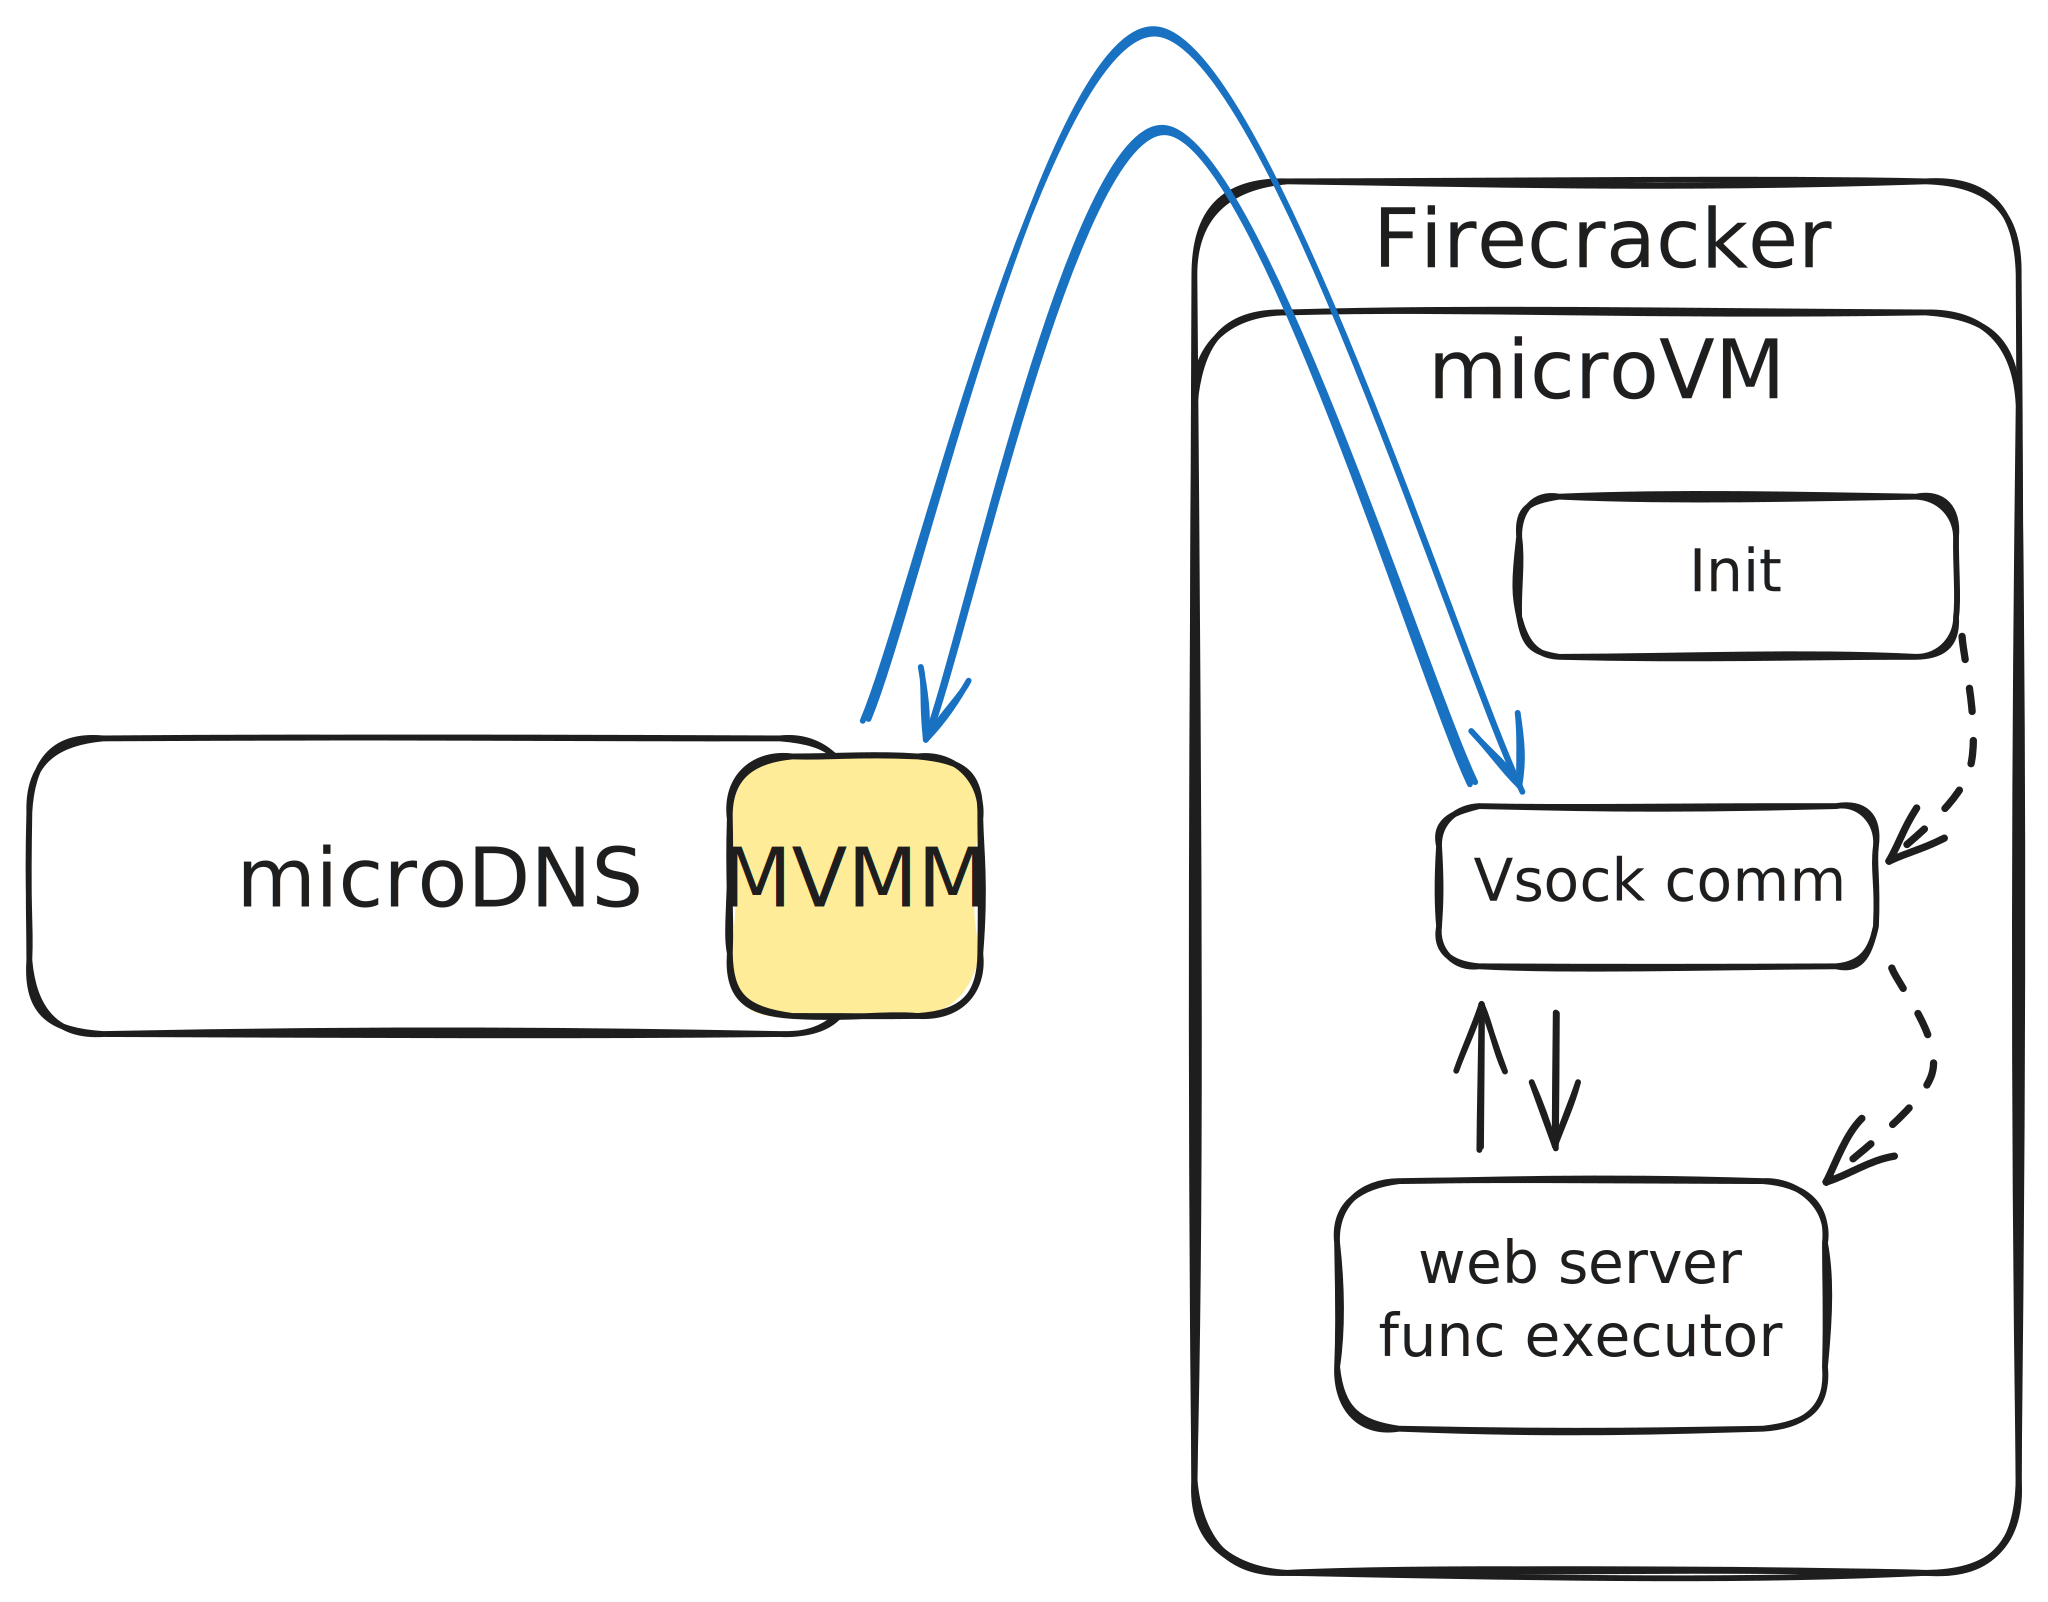
\includegraphics[width=10cm]{microVM core}
	\caption{Architecture et placement \texttt{microDNS}}
	\label{microVM:corearch}
\end{figure}

Il a été décidé donc d'avoir un init simpliste dans le microVM pour lancer les deux processus principaux.

\section{Choix d'implémentation}
\label{header:choiximpem}
L'implémentation s'est concentrée en priorité sur le cœur du mécanisme DNS.

Pour ce programme nommé "\texttt{microDNS}" qui constitue le cœur du projet avec son rôle de gestionnaire de microVM à part ses responsabilités secondaires de proxy DNS, le langage de programmation \texttt{C++} a été choisi pour plusieurs raisons. De manière générale, ce choix était principalement dicté par la capacité d'opération bas niveau du \texttt{C++} tout en fournissant des facilités haut niveau que ce soit les fonctionnalités du langage lui même ou encore les structures de données et les algorithmes proposé par sa bibliothèque standard. Pour tous les aspects fondamentales du rôle de ce programme centrale, comme la manipulation des sockets et des accès réseau, création et gestion de multiples processus fils (les instances Firecracker), la création et la configuration des périphériques virtuels de réseau \texttt{TUN/TAP} ainsi que des accès binaires avancés pour la manipulations des paquets DNS rendait juste l'utilisation d'un langage garantissant un contrôle fin et nuancé de tous ses aspects comme le \texttt{C}. Pourtant comme dit, le \texttt{C++} était préférable pour accélérer le développement grâce à ses structures de données qui permettait de se concentrer mieux sur le cœur du problématique dans les mains au lieu de passer du temps à tout recréer de zéro et surtout passer du temps à tout tester pour s'assurer que les briques de bases étaient solides. Les facilités comme les expressions régulières et la programmation orienté objet du \texttt{C++} étaient aussi des facteurs considérés pour accélérer la programmation. Il est à noter que pour des contraintes de performance et d'extensibilité, une architecture multithreadé a été envisagé qui était possible d'implanter aisément en \texttt{C++} grâce à ses performances de base déjà très à point ainsi que la manipulation et la synchronisation des threads simple. Enfin, il faut mentionner que \texttt{Java} a aussi été considéré brièvement mais un langage plus bas niveau était plus adapté pour les raisons citées.

\begin{itemize}
    \item \textbf{Composant DNS personnalisé (`microDNS`)} : Un serveur/proxy DNS a été développé en C++. Le code source principal se trouve dans \texttt{dns/}. Il met en œuvre plusieurs classes clés :
        \begin{itemize}
            \item \texttt{ConfigLoader} : Pour charger la configuration à partir d'un fichier (par exemple, `./microDNS.conf`).
            \item \texttt{MessageQueue} : Pour la communication asynchrone "thread safe" entre les différents modules du composant DNS.
            \item \texttt{QueryReceiver} : Responsable de la réception des requêtes DNS entrantes.
            \item \texttt{QueryForwarder} : Chargé de transmettre les requêtes DNS (soit à un résolveur externe, soit potentiellement au module d'orchestration interne).
        \end{itemize}
    Cette structure permet une architecture modulaire et thread-safe pour le traitement des requêtes DNS.
    \item \textbf{Préparation pour Firecracker} : Bien que l'orchestration Firecracker n'ait pas été implémentée, une configuration type pour une microVM a été définie dans le fichier \texttt{firecracker/vm\_test\_config.json}. Ce fichier spécifie les paramètres essentiels comme l'image du noyau (\texttt{vmlinux}), les arguments de démarrage, la configuration du disque racine (\texttt{rootfs.ext4}), le nombre de vCPUs, la mémoire, et l'interface réseau. Cela constitue une première étape indispensable vers l'intégration de Firecracker.
\end{itemize}
Les efforts se sont donc portés sur la mise en place d'une fondation solide pour la partie DNS, qui est cruciale pour le fonctionnement de l'ensemble du système envisagé.

\section{Difficultés}
Le but de réutiliser \texttt{systemd-resolved} et insérer \texttt{microDNS} dans la chaine de traitement DNS du système avec le moins d'impacte à sa configuration était très très difficile. Les comportements de \texttt{systemd-resolved} se sont avérés très complexes et difficile à controler.

La mise en place d'un environnement de travail et de développement a pris beaucoup trop de temps et d'effort. J'ai un Mac Intel de l'année 2018 et c'est le seul ordinateur que j'ai. Il me fallait un environnement Linux donc j'ai du passer par une machine virtuelle vu que je ne pouvais pas toujours venir dans les salles informatique du campus. Pourtant il me fallait un logiciel de virtualisation avec un support de virtualisation imbriquée. Il s'avere que sur les Mac Intel, il y a un et un seul logiciel avec ce support qui est tout récemment dévenu gratuit pour l'utilisation individuelle par chance. Cela m'a pris du temps à trouver et mettre en place.

Comprendre le sujet du projet et par la suite idéologie de Firecracker vis à vis des demandes du sujets étaient très difficile à comprendre. Et au moment où j'ai enfin compris, il me restait plus beaucoup de temps dans le projet.

\section{Fonctionnalités complétées}
Malgré les contraintes, une partie significative du projet, axée sur le composant DNS, a pu être menée à bien :

\begin{itemize}
    \item \textbf{Fondations du proxy/serveur DNS personnalisé (\texttt{microDNS})} : Le cœur du système de traitement des requêtes DNS a été implémenté en C++. Cela inclut :
        \begin{itemize}
            \item La capacité de recevoir des requêtes DNS.
            \item Un mécanisme de transmission (forwarding) des requêtes DNS, géré par la classe \texttt{QueryForwarder}.
            \item L'utilisation de files de messages (`MessageQueue`) pour une gestion asynchrone et découplée des tâches au sein du proxy.
            \item Un système de chargement de configuration (\texttt{ConfigLoader}) permettant de paramétrer le comportement du proxy via un fichier externe (\texttt{microDNS.conf}).
        \end{itemize}
    \item \textbf{Définition de la configuration des microVMs Firecracker} : Le fichier \texttt{vm\_config.json} a été créé, spécifiant une configuration de base pour les microVMs. Cela démontre une préparation pour la partie orchestration, même si son implémentation n'a pas été finalisée.
    \item \textbf{Structure générale du projet et outillage de base} : Le projet a été initialisé avec une structure de dossiers (par exemple, \texttt{dns}, \texttt{firecracker}, \texttt{report}) et les fichiers de base nécessaires.
\end{itemize}
Ces éléments constituent une base fonctionnelle pour la partie DNS, qui est la première étape essentielle vers la réalisation de l'objectif global du projet.

\section{Fonctionnalités incomplètes}
Il ne reste plus qu'à créer des processus fils Firecracker et lancer des microVM depuis \texttt{microDNS} et plus précisement son composant \texttt{microVMManager} (pas implémenté). La configuration et le lancement des microVM a été réussi mais le couplage de ces deux parties n'a pas pu etre fait. Pour les microVM, le communiquant \texttt{Vsock} n'a pas pu etre implementé non plus.

Enfin, le monitoring et le chainage des fonctions n'a pas pu etre réalisé.

Tout ceci malheureusement par manque grave de temps pourtant des solutions ont été quand meme envisagé pour ces parties pret à implementer si le temps le permettait.

\section{Lacunes et améliorations possibles}
Le travail réalisé constitue une première étape prometteuse. Pour mener le projet à son terme et l'améliorer, plusieurs pistes peuvent être envisagées :

\begin{itemize}
	\item Les performances DNS  de \texttt{microDNS} sont médiocres lors de tests avec des nombres de requetes simultanés allants de 100 à 1000 meme en vue de son architecture mutlithreadé. Ceci pourrait etre amelioré mais en réalité ce genre de cas n'arriverait pas en local (cela revient à des requetes toutes les 10 à 1ms).
	\item Firecracker pourrait etre lancé dans un "jailer" et d'autres précations d'isolations peuvent etre prises au sein des microVM comme changement d'utilisateur vers non root, changement de racine et encore
\end{itemize}

\section{Usage}
L'utilisation du système, dans sa version finalisée telle que conçue, se décomposerait en plusieurs étapes, bien que seule la partie DNS soit actuellement fonctionnelle avec Firecracker capable d'etre lancé à la main pour tester l'execution de fonction.

Pour \texttt{microDNS}:
\begin{itemize}
	\item Aller dans \texttt{dns/}
	\item Faire \lstinline|make microDNS| pour compiler \texttt{microDNS}
	\item Aller dans \texttt{dns/scripts/}
	\item Faire \lstinline|./microDNS.sh setup| pour temporairement changer de configuration DNS pour que toute requete DNS passe par \texttt{microDNS} d'abord
	\item Revenir dans \texttt{dns/}
	\item Faire \lstinline|build/microDNS| pour lancer \texttt{microDNS}
\end{itemize}

Pour Firecracker:
\begin{itemize}
	\item Aller dans \texttt{firecracker/}
	\item Faire \lstinline|make| pour télecharger une archive du noyau Linux, une configuration de noyau Linux de base et une executable Firecracker. Cela crée ensuite le rootfs et compile le noyau. 
	\item Vous pouvez désormais faire  \lstinline|make test| pour lancer un microVM en session interactive avec "root" comme nom d'utilisateur et mot de passe vide. Faites \lstinline|reboot| au sein du microVM pour quitter.
	\item Si vous voulez tester l'execution de fonction comme le ferait \texttt{microDNS} lorsqu'il gere ces microVM, rajouter \texttt{init=/init.sh -- ./test.sh} comme paramètre boot dans le début du fichier \texttt{firecracker/vm\_test\_config.json}. Vous pouvez après relancer le microVM via \lstinline|make test|. Il suffit d'aller à l'adresse 172.16.0.2:8000 dans votre navigateur pour recevoir un message généré par la "fonction" \texttt{firecracker/functions/test.sh} lancé par le serveur web au sein du microVM.
	\item Il est à noter que pour avoir accès à internet au sein du microVM, il faut faire \lstinline|make forwarding|
\end{itemize}

\pagebreak
\nocite{*}
\bibliographystyle{IEEEtran}
\bibliography{references}

\end{document}
